\pagebreak
\section{Divers}
\label{chapter:solutionDivers}

Dans cette section, nous aborderons quelques éléments secondaires de \texttt{Source Code}.
En effet, en dehors du développement, il existe bien d'autres facettes importantes du cycle de vie\footnote{
    En anglais, ce terme est connu sous le nom de "software lifecycle". (\url{https://web.maths.unsw.edu.au/~lafaye/CCM/genie-logiciel/cycle-de-vie.htm})
} d'un logiciel : le \gls{deploiement} / la \gls{maintenance}  ...

\subsection{\texorpdfstring{\Gls{cli}}{CLI}}

Comme nous l'évoquions précédemment (cf. annexe \ref{annexe:AnalyseBiblio}), il convient de disposer d'outils pour indexer / mettre en ligne un nombre conséquent de 
\glspl{resinfo}, provenant de diverses sources, en un minimum de temps. C'est pour répondre à ce besoin que nous avons développé un \Gls{cli}, sur base du framework Yargs
(cf. section \ref{section:choixTechnologiques})\footnote{
    Comme le montre le point d'entrée du \Gls{cli}, à savoir "index.js" (que nous avons inclus dans l'annexe \ref{code:mainYargs}), il sera aisé d'ajouter de nouvelles commandes à l'avenir.
}.

\begin{figure}[H]
    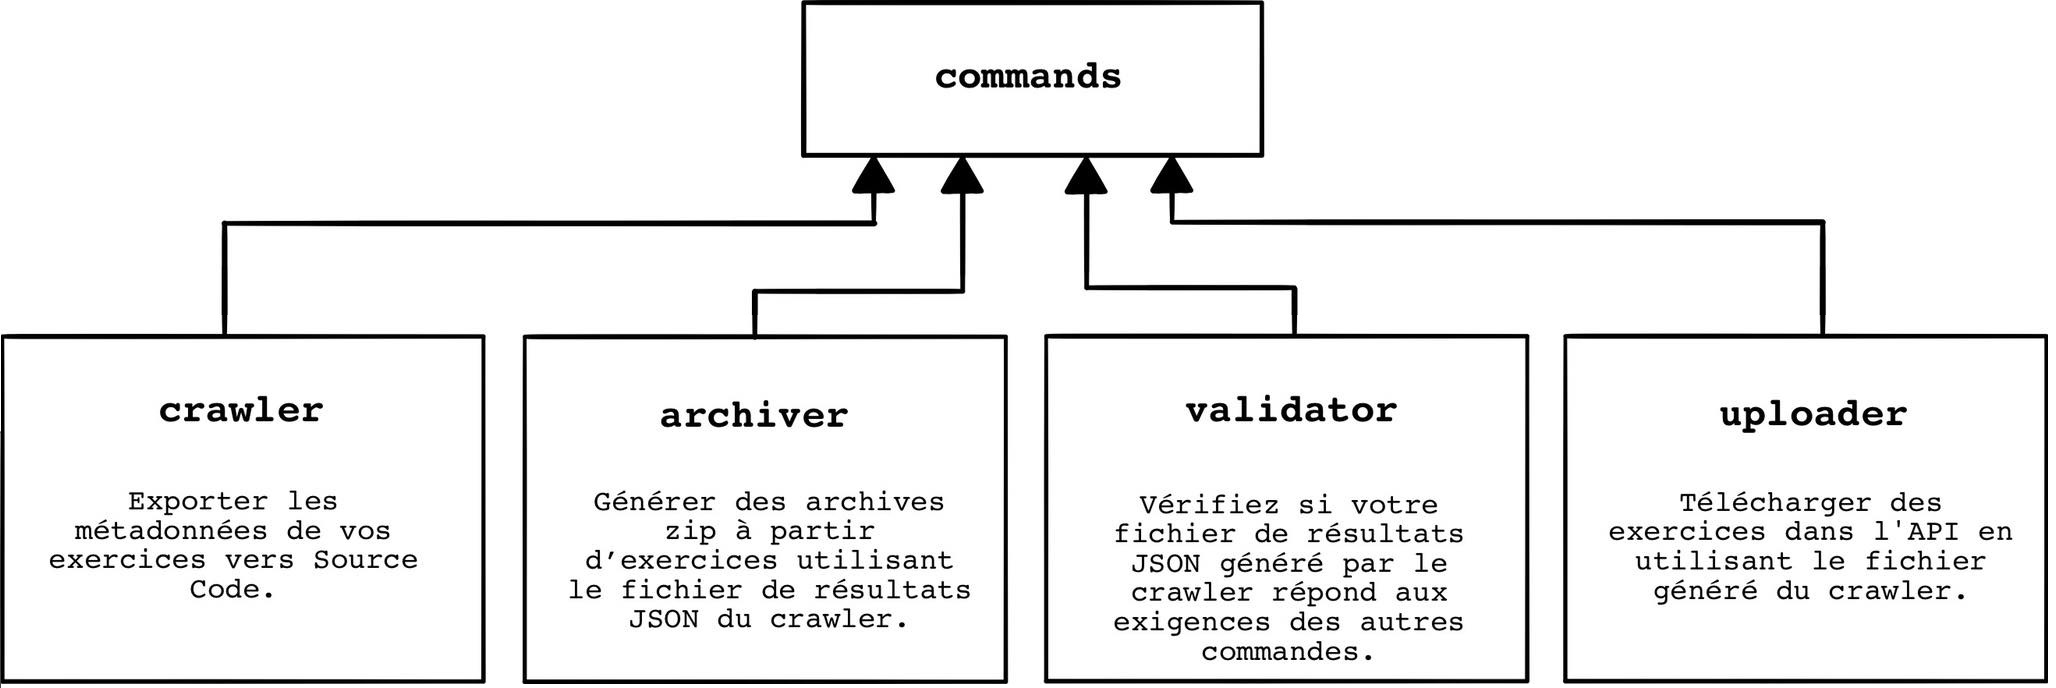
\includegraphics[width=\textwidth,height=\textheight,keepaspectratio]{images/serveur/CLI.jpg}
    \centering
    \caption{\Gls{cli} - inventaire des commandes disponibles}
    \label{fig:cliCommands}
\end{figure}

Chaque commande disposant naturellement de ses propres règles en matière d'arguments et/ou d'options.
Fort heureusement, Yargs possède un éventail de fonctionnalités très diversifié, que nous allons illustrer un échantillon représentatif sur la commande "crawler" (cf. annexe \ref{code:crawlerYargs}) :
\begin{itemize}[nosep,noitemsep,topsep=0pt,partopsep=0pt,after=\vspace*{2pt}]
    \item La possibilité d'indiquer si une option est nécessaire ou non (ligne 28)
    \item La possibilité de restreindre un choix uniquement à certaines valeurs (ligne 16)
    \item La possibilité d'identifier quels options et arguments ont été donnés à la commande (lignes 59-62)
    \item La possibilité de charger un fichier de configuration (lignes 39-40), permettant ainsi de ne pas devoir réécrire l'entièreté de la ligne de commande pour l'invoquer. 
\end{itemize}
Veuillez noter que nous avons appliqué le "principe ouvert/fermé"\footnote{
    La lettre \textbf{O} dans l'anagramme \textbf{SOLID} (\url{https://fr.wikipedia.org/wiki/SOLID\_(informatique)}), qui présente quelques principes pour la programmation orientée objet
} dans cette commande : en effet, il est possible d'utiliser des stratégies d'indexation déjà implémentées ou non (ex. "inginious-git" qui s'occupe de \glspl{resinfo} au format INGInious\footnote{
    \url{https://inginious.info.ucl.ac.be/}
}, disponibles via Git\footnote{
    \url{https://git-scm.com/}
}), tout en conservant le même comportement, quelle que soit la situation. 

Par respect de la norme que nous avons crée (cf. annexe \ref{annexe:AnalyseBiblio}), nous avons également adopté le \textbf{JSON} et les mêmes conventions d'écriture 
pour les fichiers d'entrée / de sortie des différentes commandes, à quelques exceptions près que nous avons détaillé dans le fichier README.MD. 

\pagebreak
\subsection{Docker}
\label{section:docker}

Comme expliqué par son site officiel\footnote{
    \url{https://www.docker.com/why-docker}
}, il s'agit d'une plateforme de conteneurisation permettant de paqueter une application.
Dans un conteneur sont contenus une application ainsi que tous les éléments dont elle a besoin pour fonctionner (code source, \glspl{library}, ...).
Le \gls{deploiement} pouvant être réalisé sur n'importe quelle machine, tout en restant plus léger que des alternatives existantes
\footnote{
    Des explications sont disponibles sur \url{https://www.docker.com/resources/what-container}
}.
Voici un récapitulatif des concepts clés :

\begin{figure}[H]
    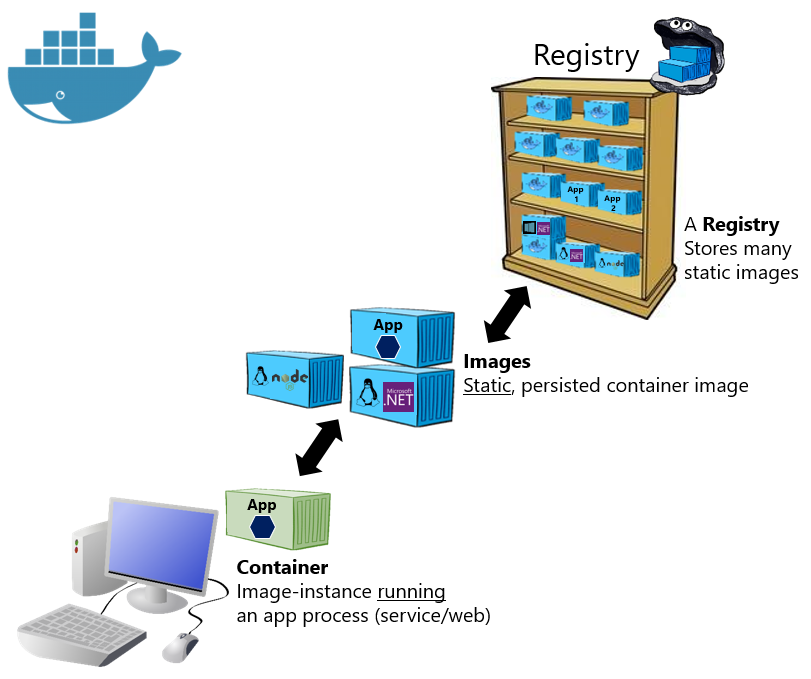
\includegraphics[width=\textwidth,height=0.38\textheight,keepaspectratio]{images/serveur/dockerTaxonomy.png}
    \centering
    \caption[Taxonomie des termes et concepts Docker]{Taxonomie des termes et concepts Docker \footnotemark}
    \label{fig:dockerTaxonomy}
\end{figure}
\footnotetext{
    \url{https://docs.microsoft.com/fr-fr/dotnet/architecture/microservices/container-docker-introduction/docker-containers-images-registries}
}

Nous avons ainsi découpé notre application en 3 images\footnote{
    Elles sont disponibles sur Docker Hub (\url{https://hub.docker.com/}) 
    et générées sur base de fichiers Dockerfile, présents dans chaque repository Github de code.
    Notons enfin la présence dans le repository miscellaneous de fichiers docker-compose-***.yml pour déployer automatiquement l'entièreté de \texttt{Source Code} avec Docker Compose, en fonction de l'environnement souhaité (plus d'informations dans le README.MD).
} :

\begin{itemize}[nosep,noitemsep,topsep=0pt,partopsep=0pt,after=\vspace*{2pt}]
    \item sourcecode-front : le \gls{frontend} de \texttt{Source Code}
    \item sourcecode\_api : le \gls{backend} de \texttt{Source Code}
    \item sourcecode-postgres : une base de données en Postgresql, contenant des données extraites par le \Gls{cli}, pour la démonstration de notre solution (cf. section \ref{section:validation})
\end{itemize}

\begin{figure}[H]
    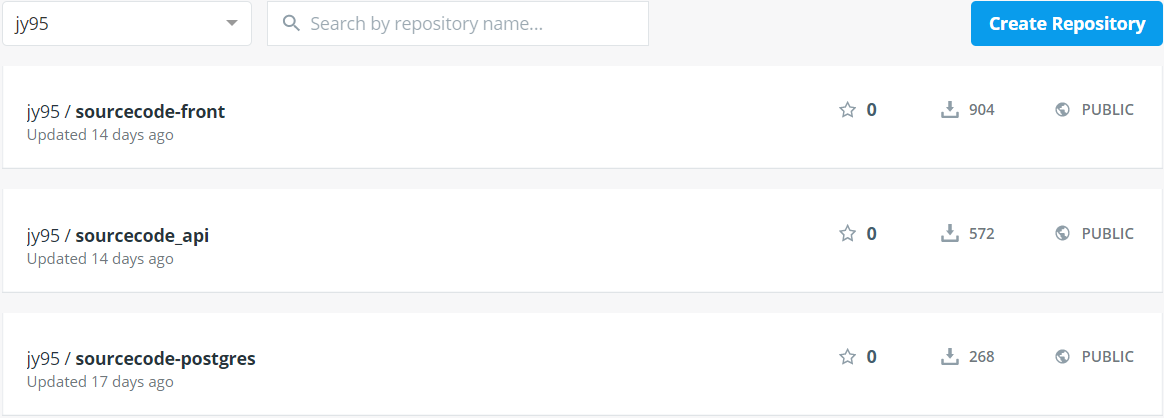
\includegraphics[width=\textwidth,height=0.15\textheight,keepaspectratio]{images/serveur/dockerHub.PNG}
    \centering
    \caption{Docker Hub - des images prêtes à l'emploi}
    \label{fig:dockerImages}
\end{figure}

\pagebreak
\subsection{Github Actions}
\label{section:GithubActions}

Vous avez peut-être noté la présence d'un dossier \textit{.github} dans chacun des repositories composant notre solution.
Pour rappel (cf. section \ref{chapter:api}), ce dossier contient des scripts permettant d'automatiser un ensemble de tâches récurrentes, par le biais de Github Actions.
Comme expliqué par Github\footnote{
    \url{https://github.com/features/actions}
}, Github Actions est une fonctionnalité permettant d'automatiser nos workflows\footnote{
    Si ce terme vous êtes inconnu, nous vous invitons à le découvrir sur \url{https://fr.wikipedia.org/wiki/Workflow}
}  
directement sur base du code hébergé chez Github (dont notamment du \gls{ci_cd}).
Ceci nous permettant de maintenir constantamment un niveau de qualité, via les quelques workflows que nous avons conçus :

\begin{itemize}[nosep,noitemsep,topsep=0pt,partopsep=0pt,after=\vspace*{2pt}]
    \item Créer une nouvelle image Docker, à chaque modification du code source (cf. section \ref{section:docker})
    \item Tester le bon fonctionnement de l'\Gls{api}, à chaque modification du code source, par le biais de tests (cf. chapitre \ref{section:validation})
    \item Vérifier la validité de la documentation en \Gls{oas}, à chaque modification du code source
    \item Générer la documentation en \textbf{HTML} (cf. figure \ref{fig:exampleDoc})
    \item Détecter et identifier les changements de l'\Gls{api} suggestibles d'impacter les clients l'utilisant, dont notamment le \gls{frontend}
    \item Compiler les sources \textbf{LaTeX} du mémoire pour générer un \textbf{PDF}
\end{itemize}

\begin{figure}[H]
    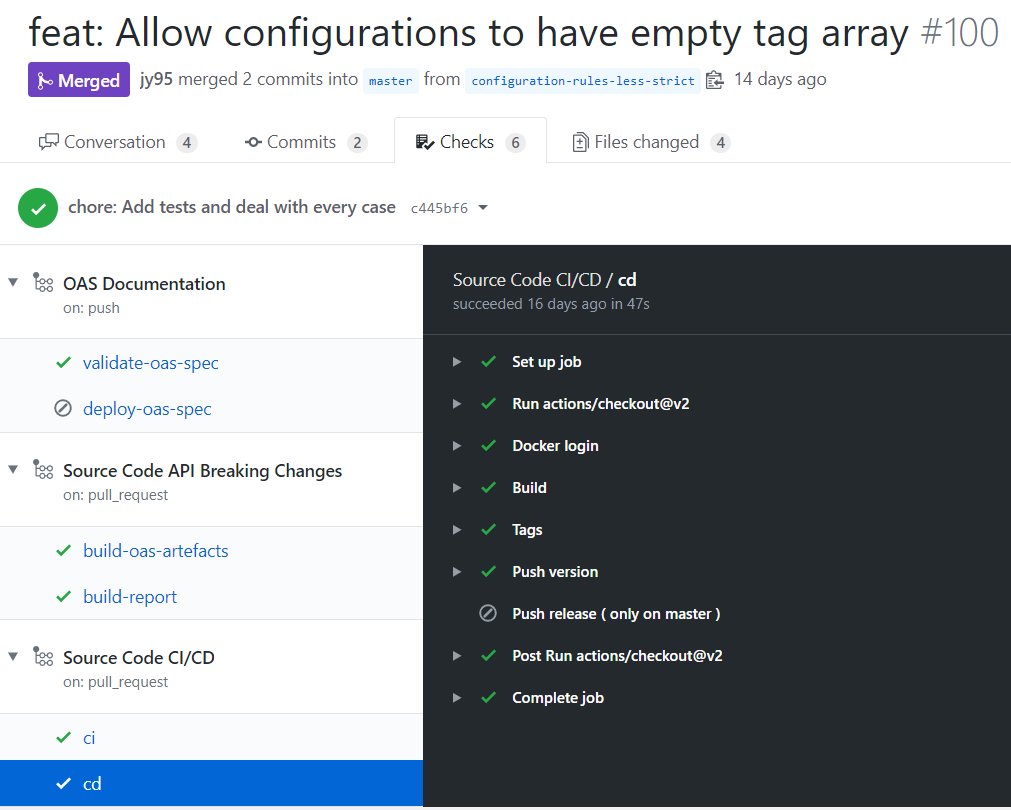
\includegraphics[width=\textwidth,height=\textheight,keepaspectratio]{images/serveur/workflowGithubActions.PNG}
    \centering
    \caption{Github Actions - exemple de workflows}
    \label{fig:GithubActionsExample}
\end{figure}